\begin{frame}
\frametitle{Pas de temps local / Classes de pas de temps}
\vskip-1em
\begin{columns}
\column{0.5\textwidth}
Configuration usuelle :
\begin{itemize}
\item [$\mathcal{C}_i$] : classe de pas de temps $i$ ;
\item [$\mathcal{T}_i$] : mailles tampon entre les classes $\mathcal{C}_i$ et $\mathcal{C}_{i + 1}$.
\end{itemize}
\vfill
Le pas de temps de la classe $\mathcal{C}_i$ est donné par $2^i \dt$, où $\dt$ est le pas de temps de la maille la plus contraignante.
\column{0.5\textwidth}
\begin{figure}
	\centering
		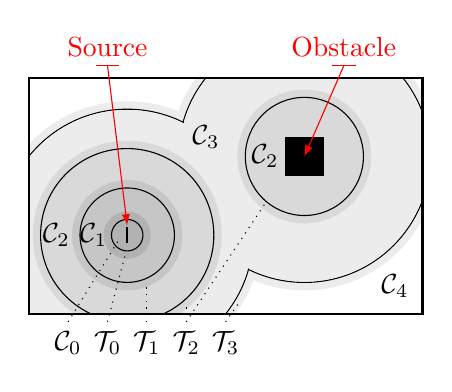
\begin{tikzpicture}[scale=0.5]
		
		\begin{scope}
			\clip (0,0) rectangle (10,6);
			
			% T4
			\draw (9.3,0.7) node {$\mathcal{C}_4$};
			
			% R3
			\fill[gray!15] (7,4) circle (3.4);
			\fill[gray!15] (2.5,2) circle (3.4);

			% T3
			\draw[] (7,4) circle (3.2);
			\draw[] (2.5,2) circle (3.2);
			\fill[gray!15] (7,4) circle (3.18);
			\fill[gray!15] (2.5,2) circle (3.18);
			\draw (4.5,4.5) node {$\mathcal{C}_3$};

			%---------------------
			% obstacle
			%---------------------
			% R2
			\fill[gray!30] (7,4) circle (1.7);

			% T2
			\draw[fill=gray!30] (7,4) circle (1.5);
			\draw (6,4) node {$\mathcal{C}_2$};
			
			%---------------------
			% source
			%---------------------
			% R2
			\fill[gray!30] (2.5,2) circle (2.4);
			
			% T2
			\draw[fill=gray!30] (2.5,2) circle (2.2);
			\draw (0.7,2) node {$\mathcal{C}_2$};
			
			% R1
			\fill[gray!45] (2.5,2) circle (1.4);
			
			% T1
			\draw[fill=gray!45] (2.5,2) circle (1.2);
			\draw (1.65,2) node {$\mathcal{C}_1$};

			% R0
			\fill[gray!60] (2.5,2) circle (0.6);
						
			% T0
			\draw[fill=gray!60] (2.5,2) circle (0.4);
		\end{scope}
		\draw[thick] (0,0) rectangle (10,6);

		% T0
		\draw (1,-0.2) node[below] {$\mathcal{C}_0$};
		\draw[dotted] (1,-0.2) -- (2.3,1.9);
	
		% R0
		\draw (2,-0.2) node[below] {$\mathcal{T}_0$};
		\draw[dotted] (2,-0.2) -- (2.45,1.5);
		
		% R1
		\draw (3,-0.2) node[below] {$\mathcal{T}_1$};
		\draw[dotted] (3,-0.2) -- (3,0.8);
		
		% R2
		\draw (4,-0.2) node[below] {$\mathcal{T}_2$};
		\draw[dotted] (4,-0.2) -- (4,0.3);
		\draw[dotted] (4,-0.2) -- (6,2.8);
		
		% R3
		\draw (5,-0.2) node[below] {$\mathcal{T}_3$};
		\draw[dotted] (5,-0.2) -- (5.35,0.3);
				
		% Source
		\fill (2.47,1.8) rectangle (2.53,2.2);
		\draw (2,6.3) node[red,above] {Source};
		\draw[-,red] (1.7,6.3) -- (2.3,6.3); 
		\draw[-,red,arrows={-latex}] (2,6.3) -- (2.5,2.25);
		
		% Obstacle
		\fill (6.5,3.5) rectangle (7.5,4.5);
		\draw (8,6.3) node[red,above] {Obstacle};
		\draw[-,red] (7.7,6.3) -- (8.3,6.3); 
		\draw[-,red,arrows={-latex}] (8,6.3) -- (7,4);

		\end{tikzpicture}
\end{figure}
\end{columns}
\vskip+1em
Résultats sur un cas d'application vu dans la dernière section pour 4 classes de pas de temps :
\begin{itemize}
\item Accélération théorique selon les classes : 4 ;
\item Facteur d'accélération de 2.84 à l'ordre $\Deg = 2$ (si $\dt$ identique) ;
\item Facteur d'accélération de 3.44 à l'ordre $\Deg = 1$ (si $\dt$ identique) ;
\item Le facteur d'échelle n'est que d'ordre 100 contre 1300 pour le corps humain, soient potentiellement 11 classes de pas de temps : accélération théorique bien supérieure.
\end{itemize}
\vfill
\end{frame}

